\documentclass[Main]{subfiles}
\begin{document}


\section{System components}

In Figure \ref{fig:ComponentsAndInterfaces} an overview of the complete system's components and interfaces is shown.
Each component and interface will described and linked with system requirements in the following subsections.

\begin{figure}[H]
\centering
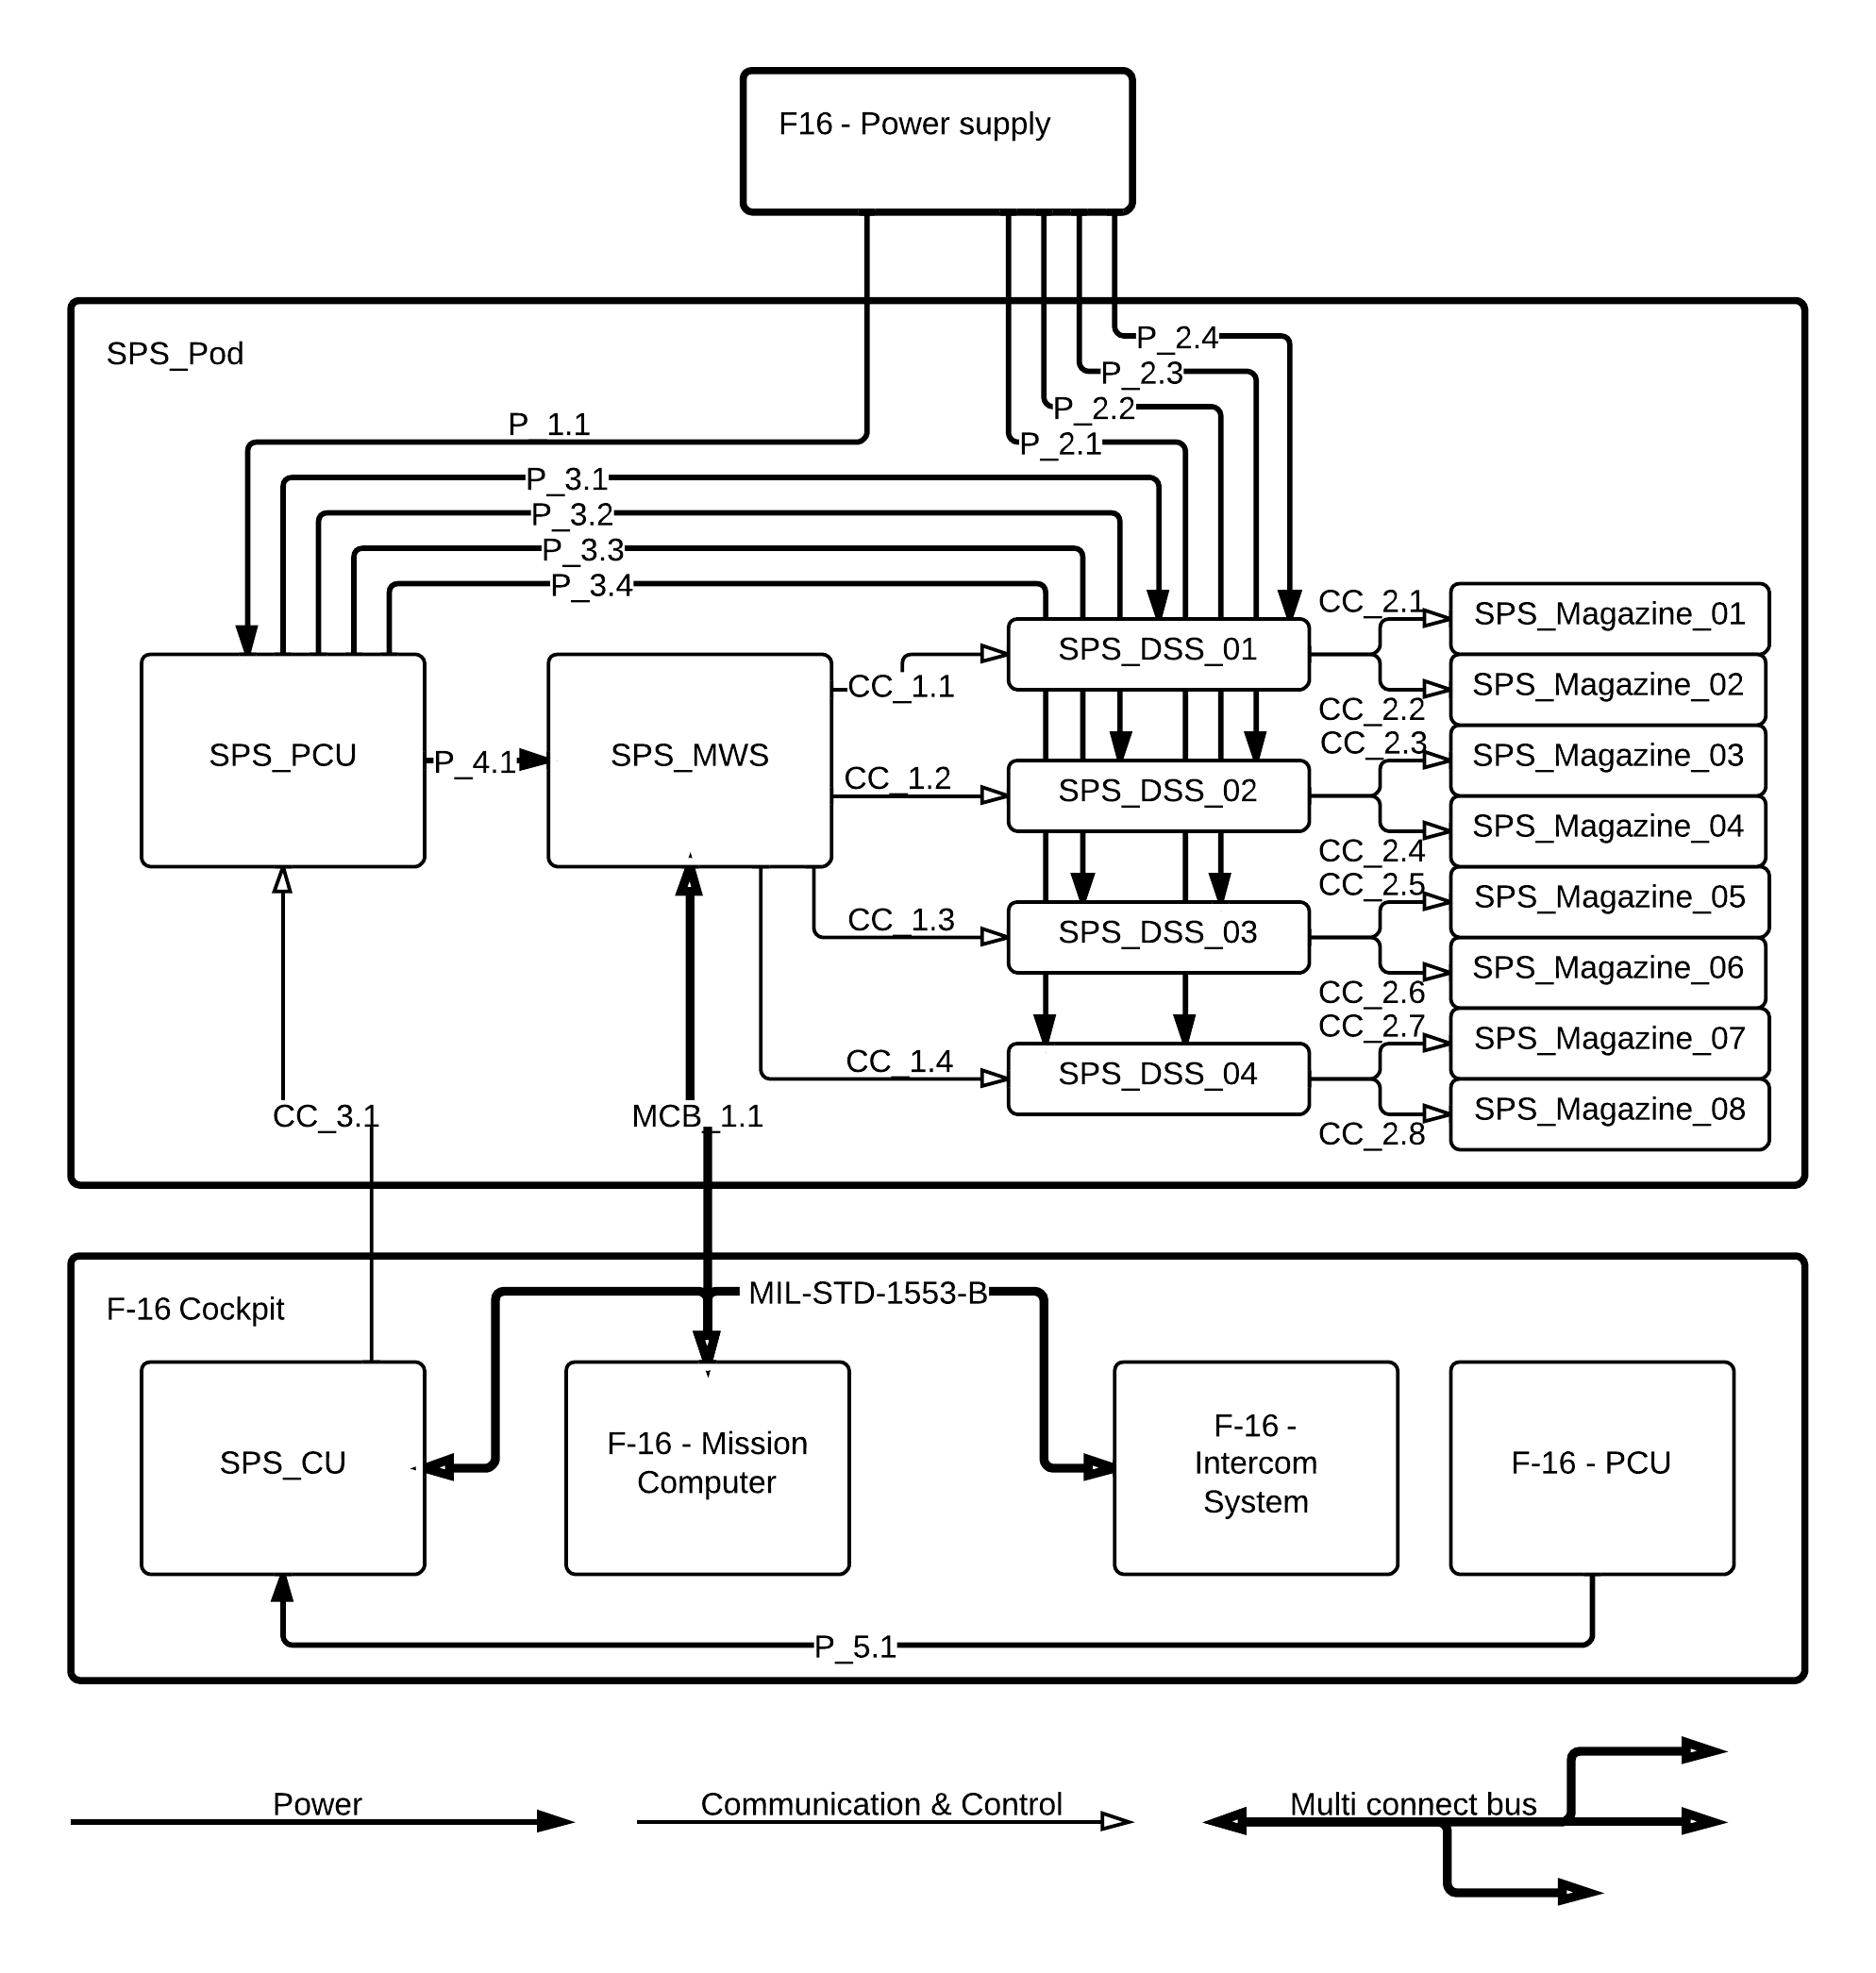
\includegraphics[width = 0.9\textwidth]{ComponentsAndInterfaces}
\caption{Components and interfaces}
\label{fig:ComponentsAndInterfaces}
\end{figure}

\subsection{SPS\_PCU}
The Power Conditioning Unit is responsible for receiving high voltage AC power from the F-16 power supply, converting it to low voltage DC power and distributing it to the MWS and the DSS's.

\subsection{SPS\_MWS}
The Missile Warning System is responsible for monitoring the planes surroundings for incoming missiles.
When a missile is identified as being in the path of the plane, the MWS will signal the cockpit unit in order to let the pilot take appropriate action.

\subsection{SPS\_DSS\_XX}
The Digital Sequencer Switches are responsible for powering and firing chaff/flare magazines on command from the MWS.

\subsection{SPS\_Magazine\_XX}
The magazines contains the payloads to be dispensed.

\subsection{SPS\_CU}
The Cockpit Unit receives input from the pilot and communicates with the MWS and the mission computer.

\end{document}
